\chapter{Análisis}
\label{chap:analisis}

En este capítulo se expondrán los requisitos obtenidos tras el estudio de las necesidades que debe cubrir la aplicación
y se elaborarán las historias de usuario asociadas.

\section{Requisitos funcionales}
\label{sec:analisis_requisitos_funcionales}

Para la definición de los requisitos funcionales que debe cumplir la aplicación, se ha hecho uso de las historias de usuario.
Esta técnica permite definir los requisitos de una forma más cercana al usuario, ya que se centra en la descripción
de las funcionalidades que este desea que tenga el sistema. Con todo, las historias de usuario obtenidas se muestran en la
Tabla \ref{tab:historias_usuario}.

\bigskip
\begin{table}[H]
  \centering
  \rowcolors{2}{white}{udcgray!25}
  \begin{tabular}{c|p{11cm}}
		\rowcolor{udcpink!25}
		\textbf{ID} & \textbf{Historia de usuario} \\\hline
		\small \textit{1} & \small Como usuario quiero poder subir mi propio dataset de textos para su perfilado \\
		\small \textit{2} & \small Como usuario quiero conocer ejemplos del formato de los datasets aceptados \\
		\small \textit{3} & \small Como usuario quiero poder seleccionar el algoritmo de perfilado que se va a utilizar \\
		\small \textit{4} & \small Como usuario quiero poder visualizar los datos obtenidos tras el perfilado \\
		\small \textit{5} & \small Como usuario quiero poder ver una lista detallada de cada persona perfilada \\
		\small \textit{6} & \small Como usuario quiero poder ordenar la lista de personas por cada uno de los campos perfilados \\
		\small \textit{7} & \small Como usuario quiero poder saber como funcionan los diferentes algoritmos de perfilado disponibles \\
		\small \textit{8} & \small Como usuario quiero ver el rendimiento de los algoritmos de perfilado disponibles \\
		\small \textit{9} & \small Como usuario quiero poder reentrenar los algoritmos con diferentes datasets \\
  \end{tabular}
  \caption{Historias de usuario}
  \label{tab:historias_usuario}
\end{table}

A partir de estas historias de usuario se ha obtenido el diagrama de casos de uso que se muestra en la Figura
\ref{fig:casos_uso}.

\bigskip
\begin{figure}[H]
	\centering
	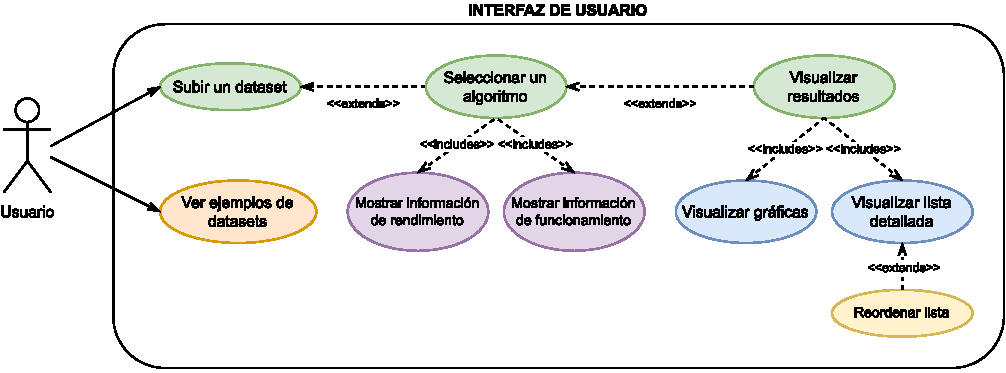
\includegraphics[width=\textwidth]{diagramas/usecases.pdf}
	\caption{Diagrama de casos de uso}
	\label{fig:casos_uso}
\end{figure}

\section{Requisitos no funcionales}
\label{sec:analisis_requisitos_no_funcionales}

Una vez definidas las funcionalidades que debe tener la aplicación, es necesario definir cuales van a ser sus requisitos
no funcionales, esto es, aquellos que están relacionados en cómo debe funcionar la aplicación. Para ello, se han tenido
en cuenta los aspectos recogidos en la Tabla \ref{tab:requisitos_no_funcionales}.

\bigskip
\begin{table}[hp!]
  \centering
  \rowcolors{2}{white}{udcgray!25}
  \begin{tabular}{c|p{9.6cm}}
		\rowcolor{udcpink!25}
		\textbf{Requisito} & \textbf{Descripción} \\\hline
		\small \textit{Usabilidad} & \small La aplicación debe ser fácil de usar, de forma que cualquier usuario pueda utilizarla sin
		necesidad de tener conocimientos previos sobre el perfilado de autores \\
		\small \textit{Escalabilidad} & \small La aplicación debe ser capaz de procesar datasets de cualquier tamaño, de forma que no
		exista un límite en el tamaño de los mismos \\
		\small \textit{Portabilidad} & \small La aplicación debe ser capaz de ejecutarse en cualquier sistema, de forma que
		los usuarios no tengan que preocuparse por el dispositivo que utilizan \\
  \end{tabular}
  \caption{Requisitos no funcionales}
  \label{tab:requisitos_no_funcionales}
\end{table}
